\chapter{Исследовательская часть}

В данной части описано проведённое исследование и его результаты, а так же технические характеристики устройства, на котором проводились замеры.

% =====================================================
\section{Технические характеристики устройства}

Технические характеристики устройства, на котором выполнялись замеры \cite{macos}:

\begin{itemize}
    \item операционная система MacOC Senoma 14.2;
    \item 18 ГБ оперативной паяти;
    \item процессор Apple M3 Pro (6 ядер производительности с частотой 4.06 ГГц и 6 ядер эффективности с частотой 2.8 ГГц).
\end{itemize}


% =====================================================
\section{Зависимость времени работы программы от глубины трассировки}

Глубиной трассировки называется максимальная глубина рекурсии при вычислении интенсивности пикселей. Чем больше глубина трассировки, тем больше отражений и преломлений учитывается в итоговой интенсивности, однако как влияет глубина трассировки на время выполнения программы?

\clearpage

В таблице \ref{tbl:research_1} представлена зависимость времени работы программы от глубины трассировки. Исследование проводилось на картинках, содержащих 1, 2 или 3 пузыря.

\begin{table}[h]
\centering
\small
\caption{Зависимость времени работы программы от глубины трассировки}
\label{tbl:research_1}
\begin{tabular}{
          |m{1.5in}|
          >{\centering\arraybackslash}m{0.7in}|
          >{\centering\arraybackslash}m{0.7in}|
          >{\centering\arraybackslash}m{0.7in}|
          >{\centering\arraybackslash}m{0.7in}|
        }
\hline
\multicolumn{1}{|c|}{Глубина трассировки} & \multicolumn{3}{c|}{Количество сфер} \\
\hline
                                      & Одна        & Две        & Три         \\
\hline
1                           &17.48&24.98&33.80\\
\hline
2                           &24.26&32.40&43.06\\
\hline
3                           &38.13&48.18&61.22\\
\hline
4                           &58.93&71.29&88.72\\
\hline
5                           &95.66&117.03&148.76\\
\hline
6                           &153.81&189.97 &227.51\\
\hline
7                           &250.60&324.76&384.53\\
\hline
8                           &419.12&559.50&643.89\\
\hline
9                           &682.20&949.00&1113.02\\
\hline
10                           &1191.09&1631.23&1889.56\\
\hline
\end{tabular}
\end{table}

\clearpage

По таблице \ref{tbl:research_1} был построен график, изображенный на рисунке \ref{img:graph}. Также на график была нанесена аппроксимация полученных значений полиномами четвертой степени.

\begin{figure}[h]
 \begin{center}
  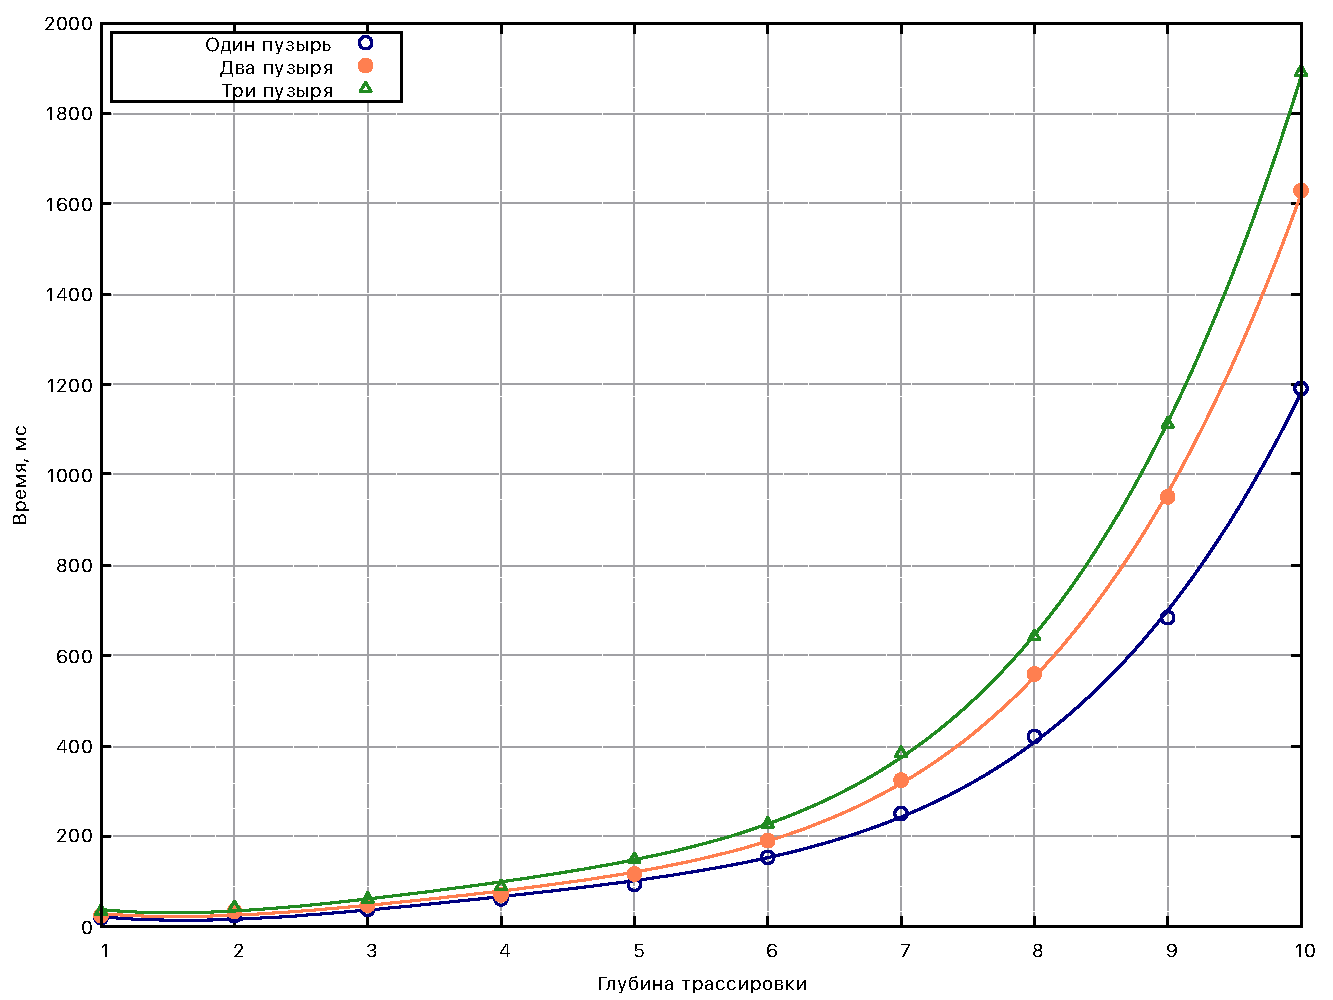
\includegraphics[width=0.9\linewidth]{img/graph.pdf}
 \end{center}
 \captionsetup{justification=centering}
 \caption{Зависимость времени работы программы от глубины трассировки}
 \label{img:graph}
\end{figure}

По итогу исследования можно сделать вывод, что при увеличении глубины трассировки возрастает время выполнения программы. Кроме того, чем больше объектов, тем быстрее растёт время выполнения программы.

%=====================================================
\section{Выводы из исследовательской части}

В исследовательской части были описаны характеристики устройства, на котором проводились замеры времени, а также проведённое исследование. Результаты исследования показывают, что с возрастанием глубины трассировки так же возрастает время выполнения программы. Кроме того, чем больше объектов на сцене, тем быстрее растёт время выполнения программы при увеличении глубины трассировки.